\documentclass[12pt]{article}\pagestyle{myheadings}
\usepackage{graphicx}
\usepackage{placeins}
\usepackage{float}
\textwidth 7.0 truein
\oddsidemargin -0.25in   %left-hand edge
\evensidemargin -0.5 truein  %right-hand edge
\topmargin -0.85in      %top of paper to top of head, pulls whole unit
\textheight 9.5in

%Enter your last name, the portfolio problem number, and the draft number.
\title{Homework 3 \\ Chaotic Dynamics - CSCI 4446}
\author{Denis Kazakov}
\date{February 1, 2015}


\usepackage{amsmath,amssymb,amsthm,amsfonts,graphicx}
%The following commands allow us to typeset theorems, propositions, definitions, etc.
\theoremstyle{plain}
\newtheorem{theorem}{Theorem}
\newtheorem{lemma}[theorem]{Lemma}
\newtheorem{corollary}[theorem]{Corollary}
\newtheorem{proposition}[theorem]{Proposition}
\newtheorem*{definition}{Definition}

\renewcommand{\qedsymbol}{\ensuremath{\blacksquare}}
\newcommand{\N}{\mathbb{N}}
\newcommand{\Z}{\mathbb{Z}}
\newcommand{\Q}{\mathbb{Q}}
\newcommand{\R}{\mathbb{R}}
\newcommand{\C}{\mathbb{C}} 
\setcounter{section}{-1}
\begin{document}
\maketitle


\section{Problem 0}

\begin{figure}[H]
\centering
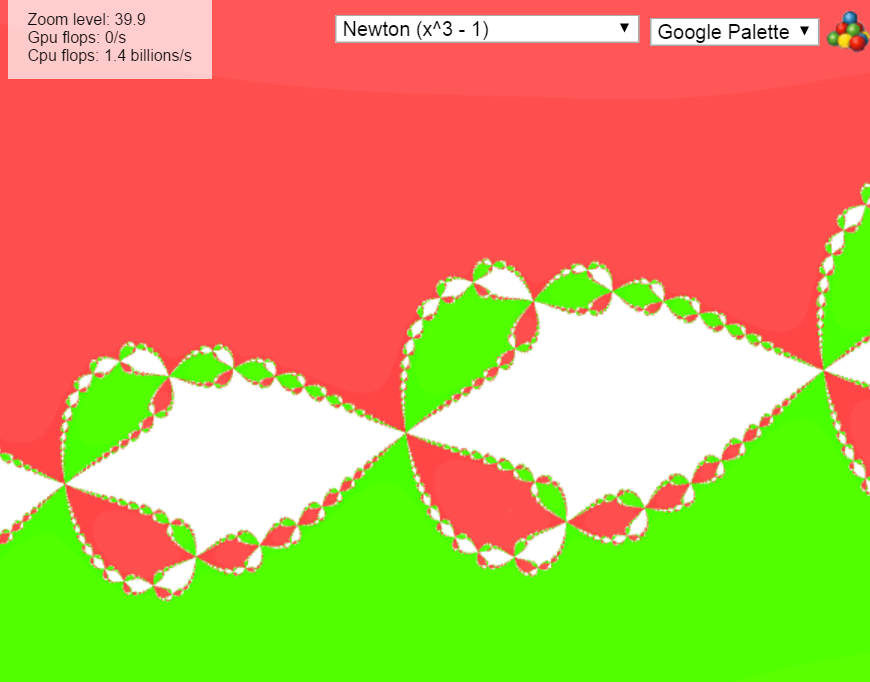
\includegraphics[scale=.4]{interesting}
\caption{$x^3 - 1 = 0$ zoomed in at 40x.}
\label{fig:my_label}
\end{figure}

It's amazing how the fractal behavior continues infinitely. 

\section{Problem 1}

$$\lim_{x\to\infty} \dfrac{\log{2^n}}{(\log{\dfrac{1}{\dfrac{5}{12}})^n}} = \lim_{x\to\infty} \dfrac{\log{2}}{\log{12/5}} \approx 0.791744069 $$

\section{Problem 2}

\subsection{a)}
$$ u_1 = x $$
$$ u_2 = \dot{u_1} = \dot{x} $$
$$ u_3 = \dot{u_2} = \ddot{x} $$
$$ \dot{u_3} = \dddot{x} = \dfrac{1}{2} (3\tan{\frac{u_3}{2}} - 16\log{u_2} + u_1) $$

Therefore, our 3 ODE's are:
$$ \dot{u_1} = \dot{x} $$
$$\dot{u_2} = \ddot{x} $$
$$\dot{u_3} = \dddot{x} = \dfrac{1}{2} (3\tan{\frac{u_3}{2}} - 16\log{u_2} + u_1) $$

\subsection{b)}

$$\dot{z} = yz + \log{y} = y\dot{y} + \log{y} = \dot{x}\ddot{x} + \log{\dot{x}} = \dddot{x}$$
Therefore, our single ODE is:
$$\dddot{x} - \dot{x}\ddot{x} - \log{\dot{x}}=0$$


\subsection{c)}

Both a)and b) ODE systems are nonlinear, because they both have a logarithmic function and tangent function in one. 

\section{3}

\subsection{a)}

\begin{figure}[H]
\centering
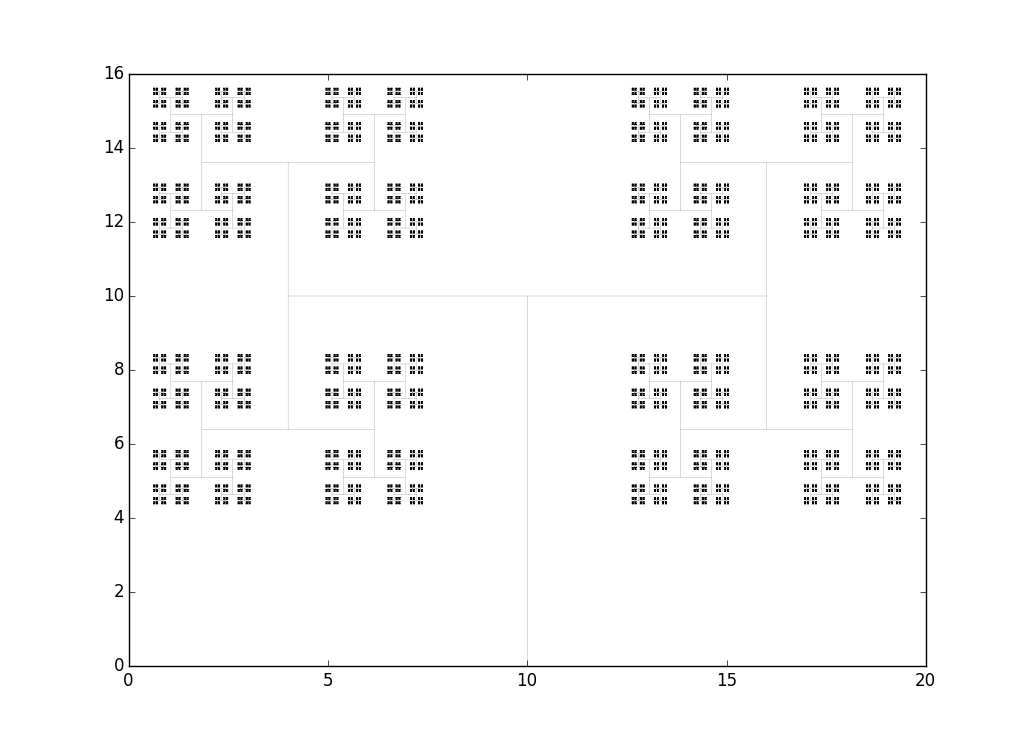
\includegraphics[scale=.3]{atree}
\caption{fractal tree with 90 degress angle}
\label{fig:my_label}
\end{figure}

\subsection{b)}

If it's half as long, then we have a tree that has all of its "children" branches being shorter than parents. Therefore, the tree "converges" to a similar shape as in part a). 

If it's $2^(\frac{1}{2})$, then each children branch is longer than its parent. Therefore, the tree "diverges". 

If we make ratio less than 0.5, then the tree would converge even faster. 

\subsection{c)}

\begin{figure}[H]
\centering
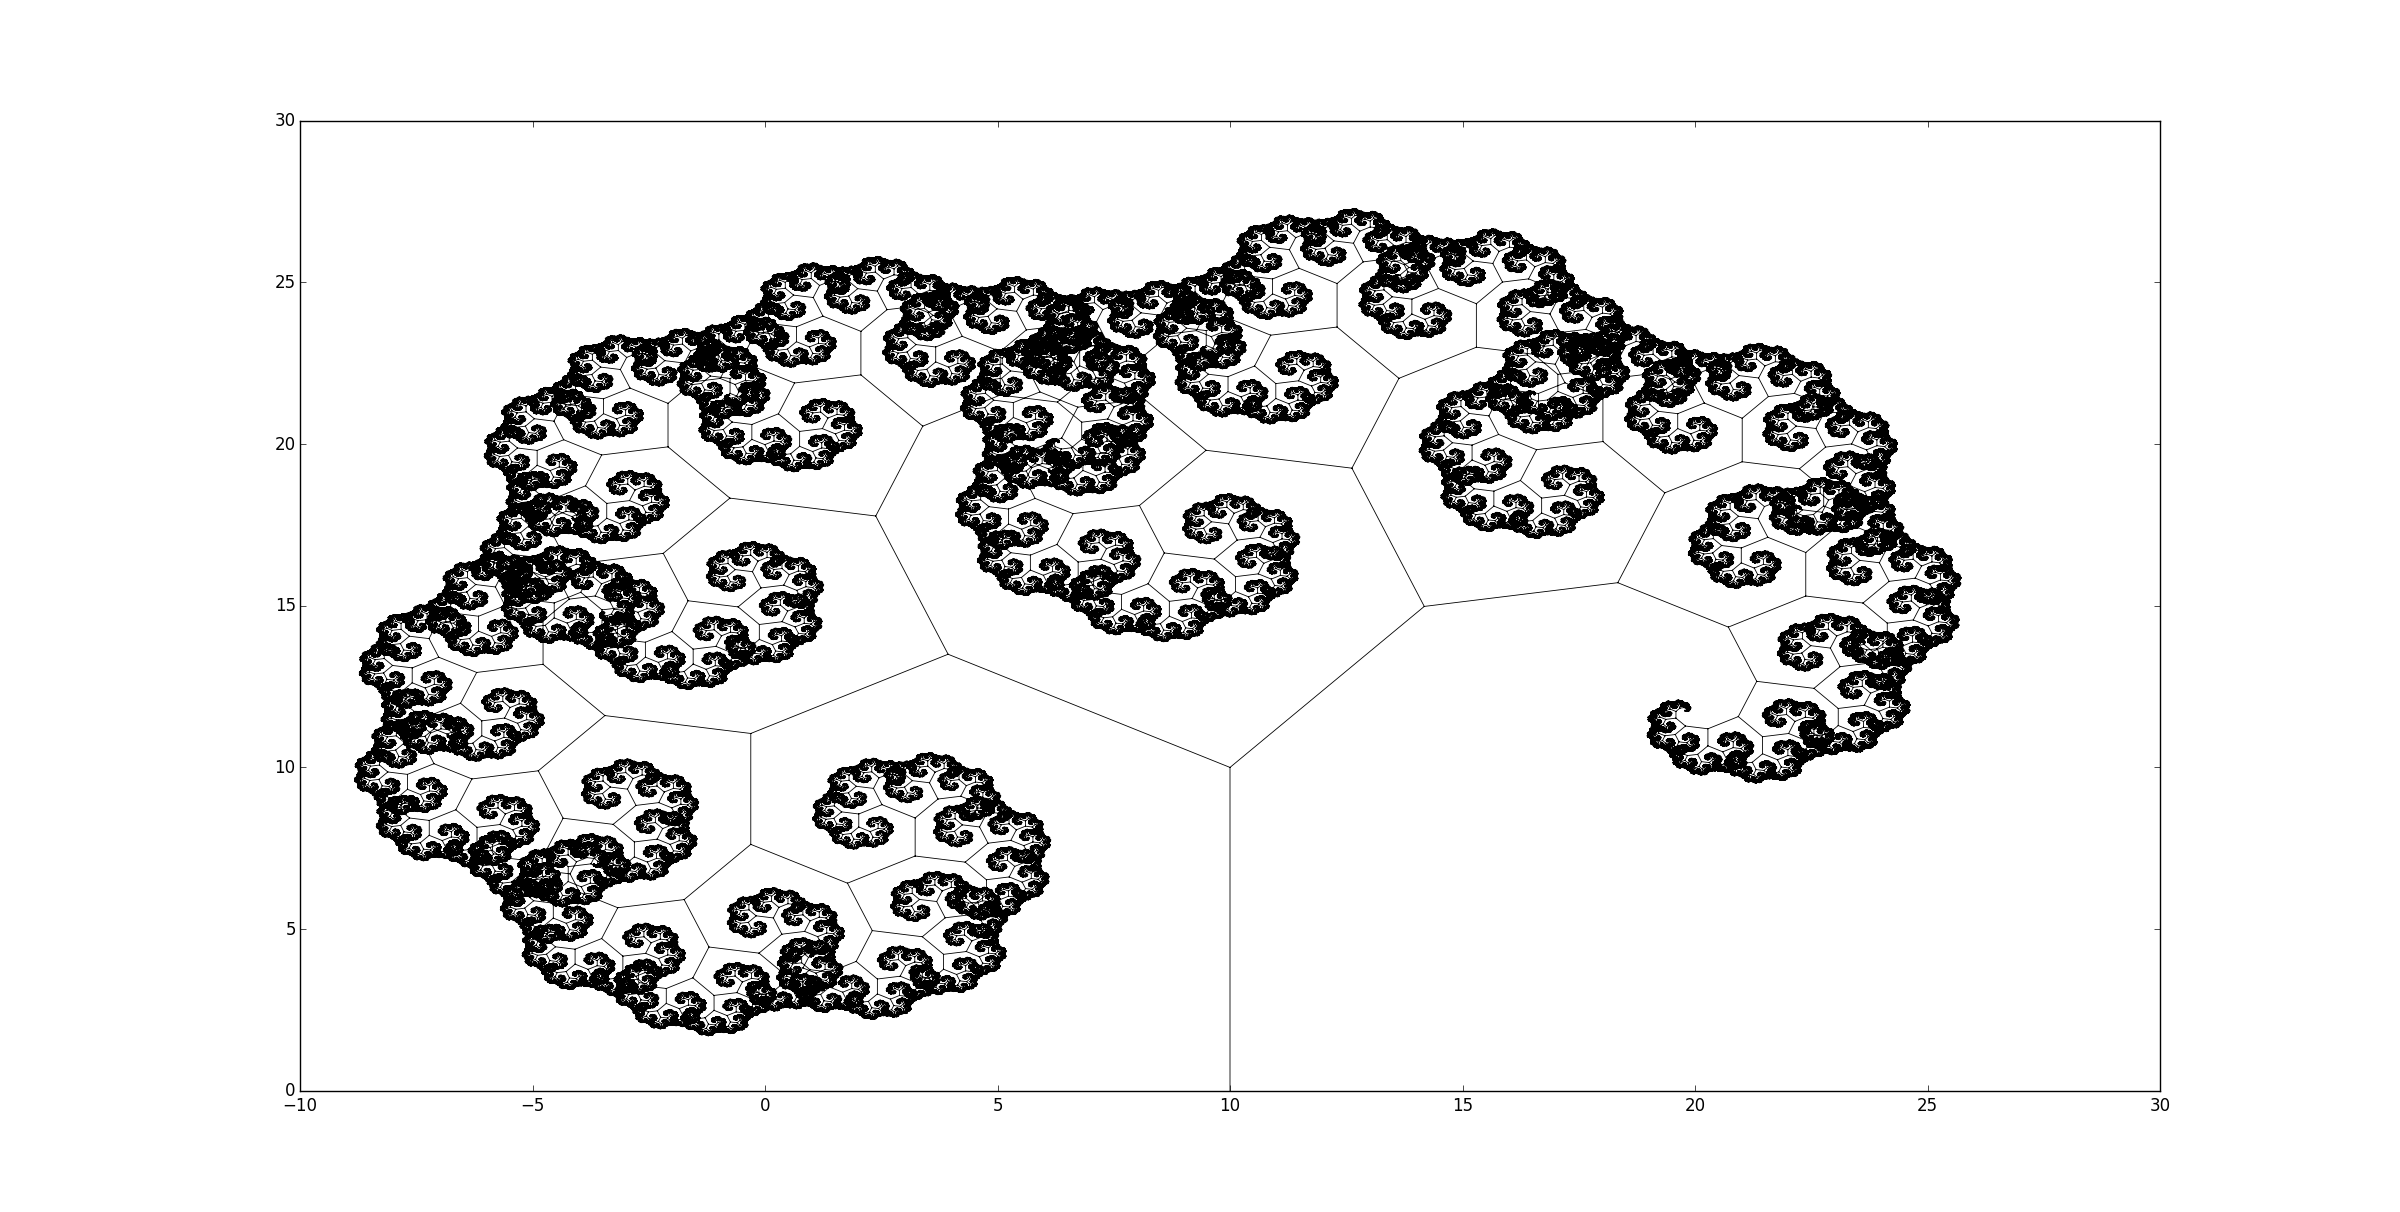
\includegraphics[scale=.2]{7_6_60_40}
\caption{LeftRatio = 0.7, RightRatio=0.6, LeftAngle = 60, RightAngle = 40}
\label{fig:my_label}
\end{figure}


\subsection{d)}

\begin{figure}[H]
\centering
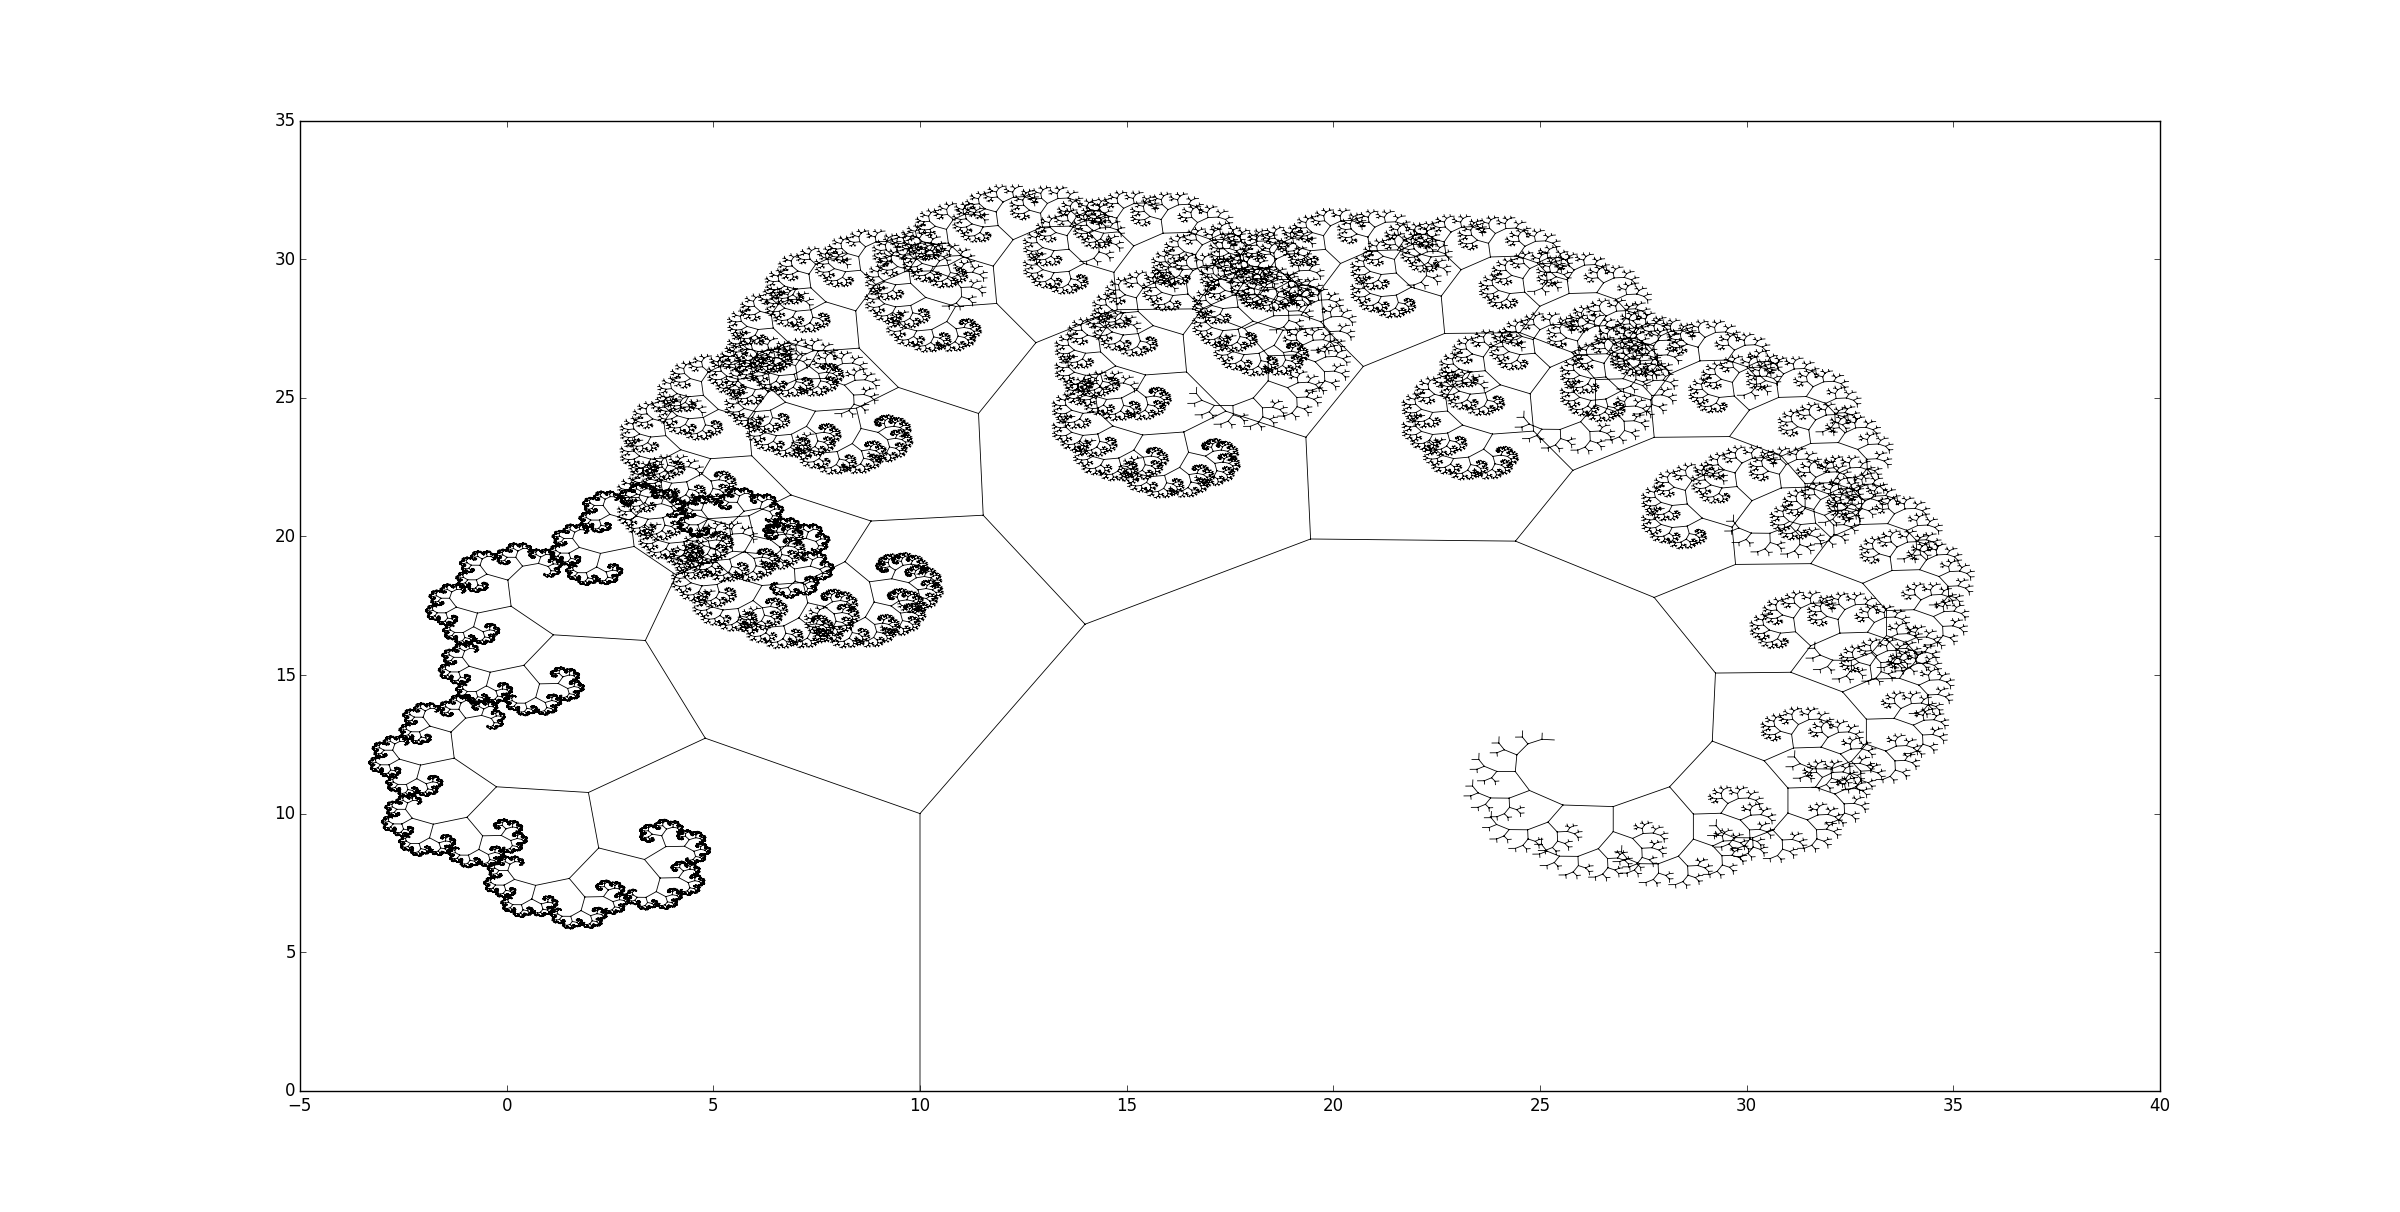
\includegraphics[scale=.2]{random_angle_length_rewriting}
\caption{Randomized lengths, angles. Rewrite them at every recursive step.}
\label{fig:my_label}
\end{figure}

\begin{figure}[H]
\centering
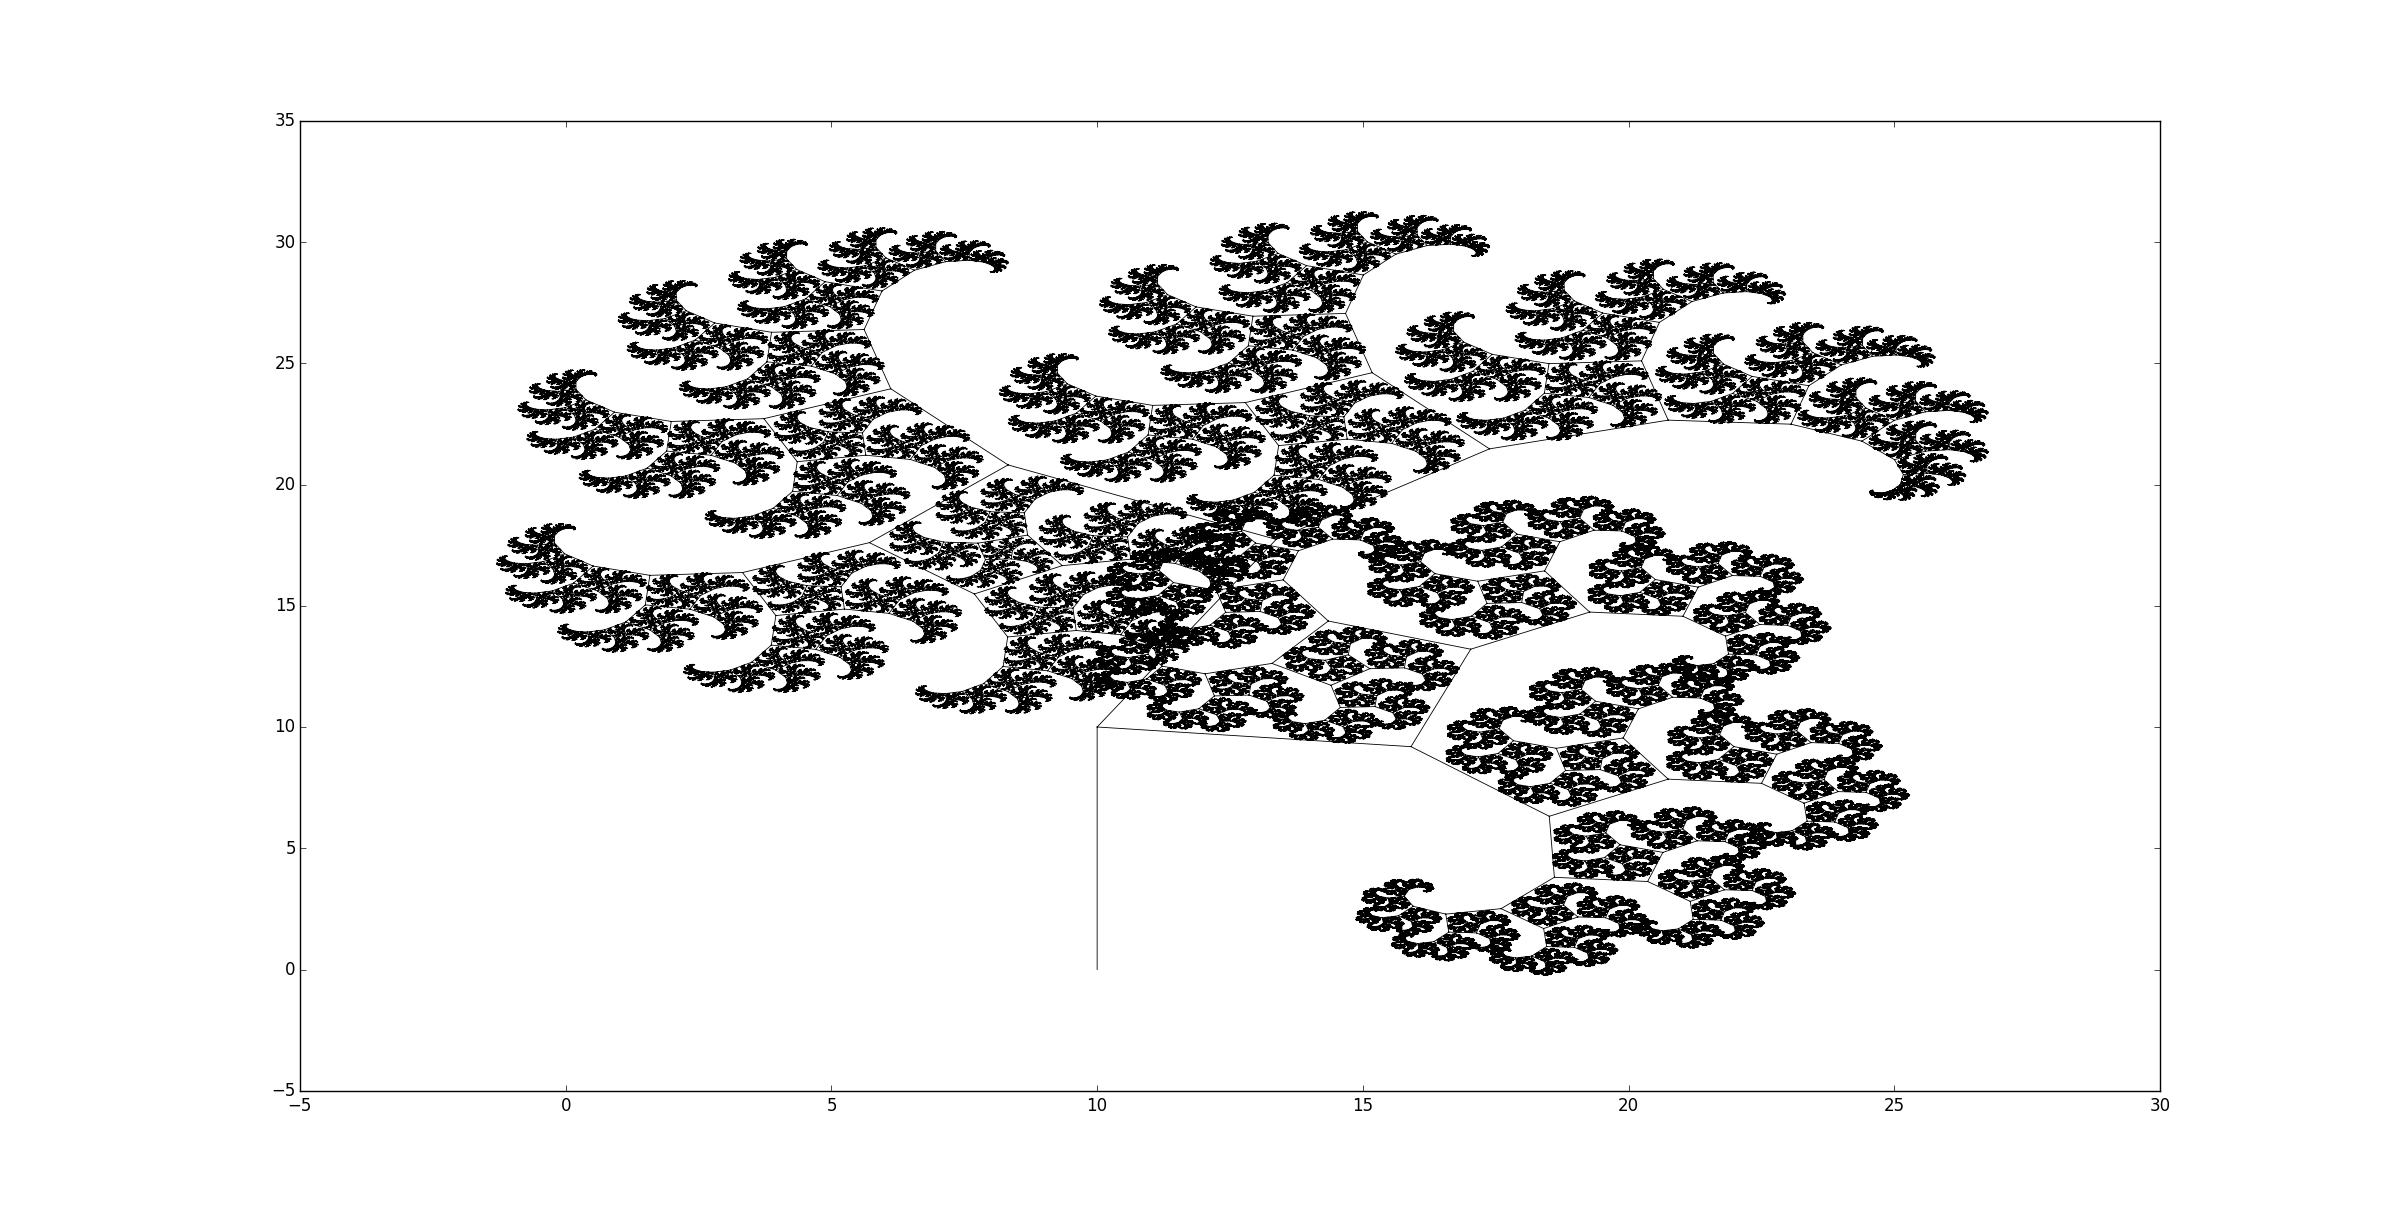
\includegraphics[scale=.15]{random_no_rewrite}
\caption{Randomized lengths, angles. Don't rewrite them at every recursive step.}
\label{fig:my_label}
\end{figure}

\end{document}